\documentclass[border=6pt]{standalone}
\usepackage{tikz}
\usetikzlibrary{arrows.meta,positioning}
\begin{document}
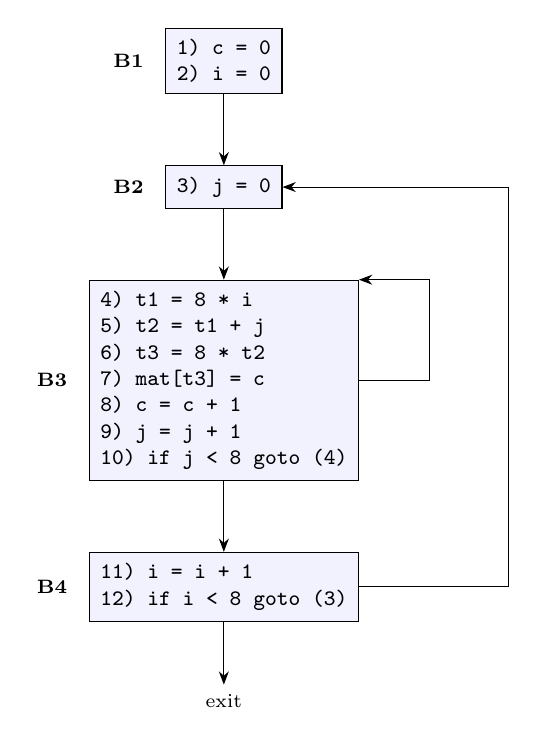
\begin{tikzpicture}[>=Stealth,font=\footnotesize,
 blk/.style={draw,align=left,inner sep=4pt,fill=blue!5,font=\ttfamily\footnotesize},
 nm/.style={font=\scriptsize\bfseries}]
\node[blk] (b1) at (0,0) {1) c = 0\\2) i = 0};
\node[blk,below=0.9cm of b1] (b2) {3) j = 0};
\node[blk,below=0.9cm of b2] (b3) {4) t1 = 8 * i\\5) t2 = t1 + j\\6) t3 = 8 * t2\\7) mat[t3] = c\\8) c = c + 1\\9) j = j + 1\\10) if j < 8 goto (4)};
\node[blk,below=0.9cm of b3] (b4) {11) i = i + 1\\12) if i < 8 goto (3)};
\node[nm,left=0.15cm of b1] {B1}; \node[nm,left=0.15cm of b2] {B2}; \node[nm,left=0.15cm of b3] {B3}; \node[nm,left=0.15cm of b4] {B4};
\node[below=0.8cm of b4,font=\scriptsize] (ex) {exit};
\draw[->] (b1) -- (b2);
\draw[->] (b2) -- (b3);
\draw[->] (b3) -- (b4);
\draw[->] (b3.east) -- ++(0.9,0) |- (b3.north east) ;
\draw[->] (b4.east) -- ++(1.9,0) |- (b2.east);
\draw[->] (b4) -- (ex);
\end{tikzpicture}
\end{document}
